%!TEX root = ../docu.tex
\section{Projektplanung}
\label{proj}
\subsection{Arbeitspakete und Planung}
Bei der Arbeit im Team stellt sich häufig die frage wie Programmfeatures Bugs und allgemeine Änderungen am Quellcode durchgeführt werden bzw. von welcher Person.

Hierfür gibt es viele Vorgehensweisen. Eine der häufigsten ist das anfertigen von sogenannten Arbeitspaketen. Diese beinhalten das vorher definierte Ziel und jene Schritte die zur Erreichung des Ziels nötig sind und welche Anforderungen das Ziel erfüllen muss.

Ein solches Arbeitspaket wird anschließend bewertet und im Aufwand eingeschätzt. Das so erstellte Arbeitspaket kann jetzt einem Bearbeiter zugeteilt werden.

Abhängigkeiten von Arbeitspaketen oder solche die auf einander aufbauen spielen eine gesonderte Rolle. Schnittstellen zwischen verschiedene in den Paketen implantierten Programmkomponenten müssen genau definiert werden und spätere Fehler oder Inkompatibilität auszuschließen.

Die Verwaltung der Pakete und Zuweisung variiert je nach Größe des Teams. Weit verbreitet sind Trac\footnote{http://trac.edgewall.org/}, Bugzilla\footnote{http://www.bugzilla.org/} sowie Redmine\footnote{http://www.redmine.org/}. Für ein Team mit kleinerer Anzahl von Mitgliedern empfehlen sich solche Systeme nicht.

Die Wartung und Konfiguration ist zu aufwendig. Die Kosten von Zeit und entstehender Nutzen stehen in keinem vertretbaren Verhältnis.

Für die Umsetzung des Projektes wurde daher auf ein Managementtool namens Trello\footnote{https://trello.com/} verwendet. es realisiert eine Management Methode namens \textit{Kanban} welche von Automobilhersteller Toyota entwickelt wurde.

\subsubsection{Kanban}

Die Funktionsweise von Kanban kann auf ein paar wesentliche Bestandteile differenziert werden. Zunächst werden Stadien definiert. Je nach Projektumgebung variieren diese Stadien. Für die Entwicklung von Anwendungen sind folgende Stadien ausreichen. Zu Beginn ist ein Paket im Stadium \textit{nicht zugewiesen} bzw. \textit{neu}. Das nächste Stadium ist \textit{zugewiesen} gefolgt vom Stadium \textit{in Bearbeitung}. Anschließend wandert das Arbeitspaket in das Stadium \textit{Test} und von dort aus in das Stadium beendet.

Das System ist sehr übersichtlich da alle Pakete auf einen Blick ersichtlich sind, sowie welche Person für das jeweilige Arbeitspaket zuständig ist.\newpage

Des Weiteren kann man sofort Erkennen in welchen Stadium sich gerade welches Paket befindet. Das ganze System ist daher sehr übersichtlich und einfach strukturiert.

Der Vorteile von Kanban liegt an der hohen Transparenz der Arbeitspakete und deren gegenwärtigen Status. Die Einführung und Umsetzung sind ressourcenschonend und schnell. Der Umgang mit Kanban ist leicht zu erlernen und gerade für kleiner Teams zu empfehlen.

\begin{figure}
\begin{center}
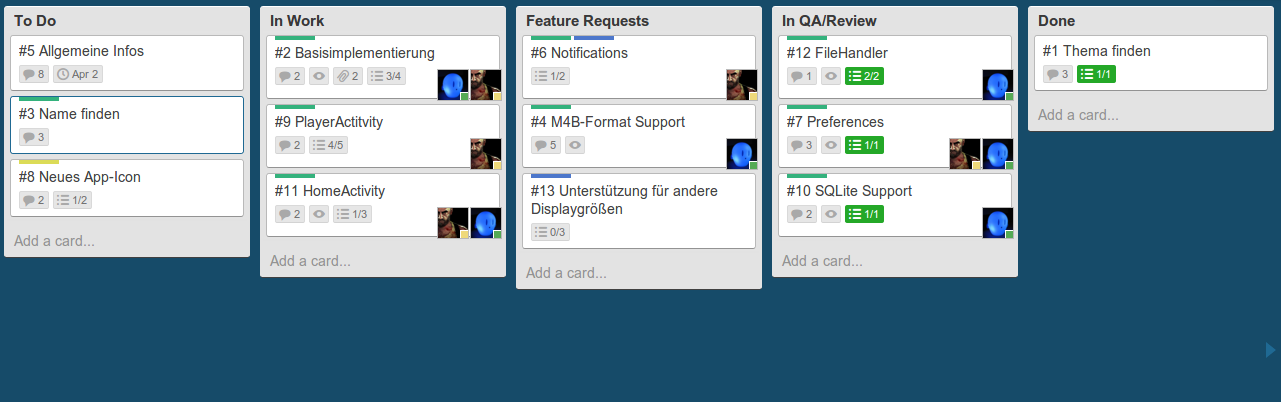
\includegraphics[scale=0.35]{images/kanban}
\caption{Kanbanboard mit verschiedneen arbeitspacketen}
\label{kanban}
\end{center}
\end{figure}

In der Abbildung \ref{kanban} ist ein Kanban-Board abgebildet. Sie durchlaufen verschiedene Stadien und wandern von der linken zu rechten Seite des Boards.

Abgeschlossene Pakete werden nach einiger Zeit vom Brett genommen um die Übersichtlichkeit weiterhin zu gewährleisten. Solche Boards können in Papierform oder auch auf elektronischen Wege simuliert werden. Eine elektronische Variante wie sie im abgearbeiteten Projekt verwendet wurde, ist genannten wurden. Weitere Einzelheiten könne aus der Literaturquelle \cite{9783898647304} entnommen werden.

\subsection{Entwicklungsumgebung}
Für das Arbeiten mit der umfangreichen Android API empfiehlt es sich eine Entwicklerwerkzeuge wie Eclipse zu wendenden. Dies gewährleistet einen schnellen Umgang mit allen Bestandteilen der Android SDK.

Des weitern können die LOG-Daten schnell ausgewertet werden und Fehler identifiziert werden. Des weiteren können ähnlich wie bei der Programmierung von Java Anwendungen Test verfasst werden und ein Debuggen erfolgen.

Eclipse bietet eine automatische Vervollständigung für Quellcode und eine Typprüfung vor der Kompilierung des Codes. Eclipse ist weiterhin in der Lage viele Codeabschnitte automatisch zu erzeugen und somit Entwicklungsschritte zu erleichtern.

Wichtig bei der Arbeit mit einer IDE\footnote{Integrated Development Environment} wie Eclipse ist die Integration des SDKs um die für die Entwicklung von Android Applikationen bereitgestellten Werkzeuge nutzen zu können. Hierzu gehören verschiedene Debuggen sowie Kompilierwerkzeuge Hilfestellung leisten sollen.

\subsection{Versionsverwaltung des Quellcode}
Die Versionierung von Quellcode spielt eine große Rolle bei der Entwicklung von Software. Hierbei werden Änderungen am Quellcode zeitlich erfasst um einen chronologischen Verlauf von Änderungen festzuhalten und die Aktualität des Codes zu gewährleisten.

Für diesen Zweck gibt es verschiedene Lösungsmöglichkeiten. Weit verbreitet sind die Versionsverwaltungssysteme SVN und GIT.
SVN ist ein zentrales Versionsverwaltungssystem für Dateien. Es gibt eine zentrale Versionierung zudem sich Klienten verbinden könne und Änderungen einreichen können.

Die Wahl für die Versionsverwaltung viel auf GIT. GIT verfolgt eine andere Strategie. Änderungen werden dezentral verwaltet. im folgenden sollen die wesentlichen Aspekte von GIT genannt werden.

\textbf{kein zentraler server}

Jeder Benutzer hat eine exakte Kopie der Versionierung und ihren verlauf. alle arbeiten können daher größtenteils ohne Netzwerkzugriff ausgeführt werden.

\textbf{Datenaustausch}

Der Austausch von Daten kann über viele Protokolle und Arten abgewickelt werden. Der Austausch ist sehr flexibel und sicher, wenn für die Übertragung geeignete, abgesicherte Protokolle verwendet werden.


\textbf{Kryptographische Sicherheit der Projektgeschichte}

Während des Versionierungprozesses wird ein eindeutiger Hash erzeugt, welcher den gesamten verlauf zur aktuellen Version widerspiegelt eine nachträgliche Änderung ist somit nicht möglich bzw. kann nicht verschleiert werden. Gelöschte Informationen bleiben erhalten und können wiederhergestellt werden.

Durch die Dezentralisierung der Versionierung muss dennoch ein Austausch der Daten zwischen den Teammitgliedern gewährleistet sein.

Hierfür gibt es verschiedene Möglichkeiten unter anderem eine gemeinsame Austauschstelle. Diese Austauschstellen fungieren als Vermittelns und Sammelpunkten. Es besteht die Möglichkeit solch einen Punkt selber zu betreiben oder kostenlose Anbieter wie GitHub\footnote{https://github.com/} zu verwenden.

